\documentclass{article}

\usepackage[spanish]{babel}
\selectlanguage{spanish}
\usepackage[utf8]{inputenc}
\usepackage[pdftex]{graphicx}

% Utilizado para recuadrar expresiones
\usepackage{amsmath}
% Recuadros con mayor separación
\setlength{\fboxsep}{6pt}

\def \anio {a\tilde{n}o}

\title{Trabajo Práctico 2\\Administración de Stocks}
\author{}
\date{\today}

%%% Agregar integrantes del grupo %%%

\begin{document}
\maketitle

%%%% Poner el enunciado aca.. y un indice %%%%
\paragraph{Ejercicio 1}
  \paragraph{Datos}
    \begin{itemize}
      \item Demanda: $d = 1000u/\anio$
      \item Costo unitario: $b = 40\$/u$
      \item Costo de setup: $K = 4000\$$ 
      \item Costo de almacenamiento: $C_1 = 540\$/u * \anio$
      \item Lead time: $LT = 2dias$
      \item Período: $T = 1\anio$
    \end{itemize}

  \paragraph{1.a}
    El modelo utilizado para representar el sistema planteado es el modelo básico con stock de reorden. Las hipótesis asumidas para ello son:
    \begin{itemize}
      \item Se administra sólo un producto.
      \item La demanda es conocida y constante.
      \item La demanda es independiente de otras variables.
      \item La reposición es instantánea.
      \item No se admite déficit del producto.
      \item El producto se mide en unidades contínuas.
      \item El horizonte de planeamiento es a largo plazo.
      \item No hay inflación.
      \item El costo de setup es independiente del tamaño del lote.
      \item El costo de almacenamiento es independiente del stock.
    \end{itemize}

  \paragraph{1.b}
        $$ q_o = \sqrt{ \frac{2KD}{TC_1}} $$
        $$ q_o = \sqrt{ \frac{2 \cdot 4000\$ \cdot 12000u/\anio}{540\$/u\cdot\anio}} $$
        $$ q_o = \sqrt{ \frac{96000000u^2}{540}} $$
        $$ \boxed{ q_o \simeq 421.63u} $$

  \paragraph{1.c}
	Dado que la fábrica tiene 20 días laborables al mes, al cabo de un año se acumulan $20 dia/mes \cdot 12 mes/\anio = 240 dia/\anio$.
        $$ \frac{T}{t_i} = \frac{D}{q} \Rightarrow t_i = \frac{Tq}{D} $$
        $$ t_i \simeq \frac{421.63u}{12000u/\anio} \simeq 0.0351\anio $$
        $$ \boxed{ t_i = 0.0351anio \cdot 240dia/\anio \simeq 8.43dias } $$

  \paragraph{1.d}
        $$ CTE_o = bD + \sqrt{ 2KDTC_1 } $$
        $$ CTE_o = 40\$/u \cdot 12000u/\anio + \sqrt{ 2 \cdot 4000\$ \cdot 12000u/\anio \cdot 540\frac{\$}{u\cdot\anio} } $$
        $$ CTE_o \simeq 480000\$/\anio + 227684\$/\anio $$
        $$ \boxed{ CTE_o \simeq 707684\$/\anio } $$

  \paragraph{1.e}
        $$ n = \frac{D}{q} \simeq \frac{12000u}{421.63u} $$
        $$ \boxed{ n \simeq 28.46 } $$

  \paragraph{1.f}
        $$ SR = LT \cdot d = \frac{2 dias}{240dias/\anio} \cdot  12000u/\anio $$
        $$ \boxed{ SR \simeq 100u } $$

  \paragraph{1.g}
	Para lograr que no quede stock remanente al finalizar el año, $n$ debe ser una cantidad entera, de manera que el último lote se acabe al finalizar este período.

	Los números enteros más cercanos al $n$ óptimo son $n_1 = 28$ y $n_1 = 29$.

	El procedimiento a seguir es obtener el $CTE$ para cada valor de $n$ y elegir el menor.

	\subparagraph{n = 28}
	$$ n = D / q $$
	$$\Rightarrow q_1 = D / n = 12000u/28 \simeq 428.57u $$

        $$ CTE_1 = b D + q_1 C_1 T / 2 + K D / q_1 $$
        $$ CTE_1 \simeq 40\$/u \cdot 12000u/\anio + \frac{1}{2} 428.57u \cdot 540\frac{\$}{u\cdot\anio} + \frac{4000\$ \cdot 12000u/\anio}{428.57u} $$
        $$ CTE_1 \simeq 707714 \$/\anio $$

	\subparagraph{n = 29}
	$$ n = D / q $$
	$$\Rightarrow q_2 = D / n = 12000u/29 \simeq 413.79u $$

        $$ CTE_2 = b D + q_2 C_1 T / 2 + K D / q_2 $$
        $$ CTE_2 \simeq 40\$/u \cdot 12000u/\anio + \frac{1}{2} 413.79u \cdot 540\frac{\$}{u\cdot\anio} + \frac{4000\$ \cdot 12000u/\anio}{413.79u} $$
        $$ CTE_2 \simeq 707724 \$/\anio $$

        Puede verse que $CTE_1 < CTE_2$, por lo tanto $ \boxed{ n = 28 } $

\paragraph{Ejercicio 2}
  \paragraph{Datos}
    \begin{itemize}
      \item Demanda: $d = 1000u/\anio$
      \item Costo unitario: $b = 40\$/u$
      \item Costo de setup: $K = 4000\$$ 
      \item Costo de almacenamiento: $C_1 = 540\$/u * \anio$
      \item Lead time: $LT = 2dias$
      \item Período: $T = 1\anio$
      \item Stock de protección: $ SP = 5dias * \frac{1000u}{20dias} = 250u$
      \item Superficie unitaria: $ SU = 2m^2/u$
      \item Superficie disponible: $ ST = 1500m^2$
    \end{itemize}

  \paragraph{2.a}
    El modelo utilizado para representar el sistema planteado es el modelo básico con stock de reorden y stock de protección. Las hipótesis asumidas para ello son:
    \begin{itemize}
      \item Se administra sólo un producto.
      \item La demanda es conocida y constante.
      \item La demanda es independiente de otras variables.
      \item La reposición es instantánea.
      \item No se admite déficit del producto.
      \item El producto se mide en unidades contínuas.
      \item El horizonte de planeamiento es a largo plazo.
      \item No hay inflación.
      \item El costo de setup es independiente del tamaño del lote.
      \item El costo de almacenamiento es independiente del stock.
    \end{itemize}

  \paragraph{2.b}
    Este sistema mantiene todos los datos del anterior y agrega un nuevo término al cálculo de $CTE$, teniendo en cuenta el costo de almacenamiento del stock de protección.
        $$ CTE = b D + q \cdot C_1 T / 2 + K D / q + SP \cdot C_1 T $$

    Como el nuevo término añadido no depende del valor de $q$, el lote de compra óptimo se mantiene igual al del ejercicio anterior.

    Sin embargo, se añade una restricción, y es que la superficie disponible limita el stock a un máximo de $\frac{1500m^2}{2m^2/u} = 750u $.

    Esto implica que $ q + SP \le 750u \Rightarrow q \le 750u - SP = 750u - 250u = 500u$

    Ya que $q_o = 421.63u \le 500u $, la nueva restricción no afecta al óptimo obtenido.
    
    Por lo tanto:
        $$ \boxed{ q_o \simeq 421.63u} $$

  \paragraph{2.c}
        $$ CTE = b D + q \cdot C_1 T / 2 + K D / q + SP \cdot C_1 T $$
        $$ CTE \simeq 40\$/u \cdot 12000u/\anio + 421.63u \cdot 540\frac{\$}{u\cdot\anio} / 2 + \frac{4000\$ \cdot 12000u/\anio}{421.63u} + 250u \cdot 540\frac{\$}{u\cdot\anio}$$
        $$ \boxed{ CTE_o \simeq 842724\$/\anio } $$


  \paragraph{2.d}
        $$ SR = SP + LT \cdot d $$
        $$ SR = 250u + \frac{2 dias}{240dias/\anio} \cdot 12000u/\anio $$
        $$ \boxed{ SR = 350u } $$

  \paragraph{2.e}
    Bajando la superficie disponible a $1100m^2$, el almacén baja su capacidad a $550u$.
    $$ q + SP \le 750u \Rightarrow q \le 550u - SP = 550u - 250u = 300u $$

    Dado que $q_o > 300u$, no se satisface la restricción de espacio. Sin embargo, teniendo en cuenta la forma de la curva que define $CTE$, se deduce que el $q \le 300u$ cuyo $CTE$ es más cercano al óptimo, es el más cercano a $q_o$, y este es el $q = 300u$.

    Bajo estas condiciones:
        $$ CTE_o = 40\$/u \cdot 12000u/\anio + 300u \cdot 540\frac{\$}{u\cdot\anio} / 2 + \frac{4000\$ \cdot 12000u/\anio}{300u} + 250u \cdot 540\frac{\$}{u\cdot\anio}$$
        $$ \boxed{ CTE_o \simeq 856000\$/\anio } $$


\paragraph{Ejercicio 3}

Los datos proporcionados en el ejercicio son los mismos que los del Ejercicio 1; es decir:
Demanda anual = $ D = 12000 u $, un lead time $ LT = 0.5479 \anio $, un costo de adquisici\'on $ b = \$40 u^{-1} $, un costo de emisi\'on de orden de compra $ k = \$4000 $, 
un costo de almacenamiento anual $ C_1 = \$540 $ y ademas un costo de agotamiento $ C_2 = \$2100 u^{-1}\anio^{-1} $

  \paragraph{3.a}
   El modelo elegido para la resoluci\'on de este problema, es el {\bf Modelo b\'asico con agotamiento}. A continuaci\'on se enuncian las hip\'otesis de dicho modelo:

  \begin{itemize}
   \item Se administra un \'unico item o producto.
   \item La demanda del producto es independiente.
   \item La demanda es conocida y constante.
   \item La reposici\'on es instantanea.
   \item El plazo de entrega es conocido y constante.
   \item No hay stock de protecci\'on.
   \item Tanto b como k como $ C_1 $ son independientes de la cantidad a pedir.
   \item No hay restricciones que limiten la cantidad del lote a pedir.
   \item El producto se mide en unidades continuas.
   \item El horizonte de planeamiento es a largo plazo.
  \end{itemize}

  \paragraph{3.b}
  Para determinar el tama\~no del lote optimo de compra se calcula $ q_o $:
  
  $$ q_o = \sqrt{\frac{2 \cdot K \cdot D}{T \cdot C_1}} \cdot \sqrt{\frac{C_1 + C_2}{C_2}} $$
  
  $$q_o = \sqrt{\frac{2 \cdot \$4000  \cdot 12000 u \anio^{-1}}{1 \anio \cdot \$540 u^{-1}\anio^{-1}}} \cdot \sqrt{\frac{\$540 u^{-1}\anio^{-1} + \$2100 u^{-1}\anio^{-1}}{\$2100 u^{-1}\anio^{-1}}} $$

  $$q_o = 421.637 u \cdot 1.121 $$

  $$ \boxed{ q_o = 472.66 u } $$

  \paragraph{3.c}
  Para calcular el tiempo de reaprovisionamiento entre dos intervalos sucesivos se calcula $t_i$. Utilizando que: $ \frac{D}{q_o} = \frac{T}{t_i} $

  $$t_i = \frac{q_o}{D} $$
  $$t_i = \frac{472.66 u}{12000 u \anio^{-1}} $$
  $$\boxed{t_i = 0.03938 \anio} $$

  \paragraph{3.d}
  Para calcular el costo total esperado \'optimo anual, se utiliza que:

  $$CTE_o = b \cdot D + \sqrt{2 \cdot K \ cdot D \cdot T \cdot C_1} \cdot \sqrt{\frac{C_2}{C_1 + C_2}} $$
  $$CTE_o = \$40 u^{-1} \cdot 12000 u \anio^{-1} + \sqrt{2 \cdot \$4000 \cdot 12000 u \anio^{-1} \cdot 1 \anio \cdot \$540 u^{-1}\anio^{-1} } \cdot \sqrt{\frac{\$2100 u^{-1}\anio^{-1}}{\$540 u^{-1}\anio^{-1} + \$2100 u^{-1}\anio^{-1}}} $$
  $$CTE_o = \$480000 + 227683.99 \cdot 0.89188 $$ 
  $$\boxed{CTE_o = \$683066.78}$$

  \paragraph{3.e}
  Para calcular el n\'umero de pedidos que habr\'a que realizar en un a\~no se calcula:
  $$n = \frac{D}{q_o} $$
  $$n = \frac{12000 u \anio^{-1}}{472.66 u} $$
  $$\boxed{n = 25.388 ordenes \anio^{-1}} $$

  \paragraph{3.f}
  La cantidad m\'axima de unidades a mantener en stock se calcula como:
  $$S_o = \sqrt{\frac{2 \cdot K \cdot D}{T \cdot C_1}} \cdot \sqrt{\frac{C_2}{C_1 + C_2}} $$
  $$S_o = \sqrt{\frac{2 \cdot \$4000 \cdot 12000 u \anio^{-1}}{1 \anio \cdot \$540 u^{-1}\anio^{-1} }} \cdot \sqrt{\frac{\$2100 u^{-1}\anio^{-1}}{\$540 u^{-1}\anio^{-1} + \$2100 u^{-1}\anio^{-1}}} $$
  $$\boxed{S_o = 376.05 u} $$

  \paragraph{3.g}
  Para calcular la cantidad m\'axima de unidades agotadas se utiliza que:
  $$S_a = q_o - S_o $$
  $$S_a = 472.66 u - 376.05 u $$
  $$\boxed{S_a = 96.61 u } $$

 \paragraph{3.h}
 El stock de reorden, considerando 20 dias laborales por mes, se calcula como:
  
 $$S_r = LT \cdot d - (q_o - S_o) $$
 $$S_r =  \frac{2dias \cdot 12000 u \anio^{-1}}{\frac{\anio}{240 dias}} - ( 472.66 u - 376.05 u) $$
 $$\boxed{S_r = 3.39 u} $$

  \paragraph{3.i}
  Para calcular lo pedido, se calculan $t_1$ y $t_2$ siendo $t_1$ el tiempo durante el cual se satisface la demanda y $t_2$ el tiempo durante el cual hay d\'eficit de producci\'on.

  $$t_1 = \frac{S_o \cdot t_i}{q_o} $$
  $$t_1 = \frac{376.05 u \cdot 0.03938 \anio}{472.66 u} $$
  $$\boxed{t_1 = 0.0313 \anio}$$

  $$t_2 = \frac{(q_o - S_0) \cdot t_i}{q_o} $$
  $$t_2 = \frac{(472.66 u - 376.05) u \cdot 0.03938 \anio}{472.66 u} $$
  $$\boxed{t_2 = 0.0080 \anio} $$
  
 
\paragraph{Ejercicio 4}
    Los datos proporcionados son la demanda anual $ D = 20000 u $, el costo de setup $ K = \$6000 $, el costo de almacenamiento $ C_1 = \$20\ u^{-1}\ \anio^{-1} $ y la tasa de producción $ p = 5000u\ mes^{-1} = 60000u\ \anio^{-1}$.

    \paragraph{4.a}
    El modelo elegido para este problema es el Modelo de Reposición no Instantánea. Se asumen las siguientes hipótesis:
        \begin{itemize}
            \item Se administra un solo producto.
            \item La demanda es conocida y constante.
            \item No hay descuentos por cantidad.
            \item No hay inflación.
            \item La producción se efectúa a tasa conocida y constante.
            \item No se admite agotamiento.
            \item No hay stock de protección.
            \item Costo de setup independiente del tamaño del lote.
            \item Costo unitario de almacenimiento independiente del stock.
            \item Se supone continuidad permanente de operación.
        \end{itemize}

    \paragraph{4.b.} 
        $$ q_o = \sqrt{ \frac{2KD}{TC_1 \left( 1 - \frac{d}{p} \right)} } $$
        $$ q_o = \sqrt{ \frac{2 \cdot \$ 6000 \cdot 20000u\ \anio^{-1}}{\$20 u^{-1}\ \anio^{-1} \left( 1 - \frac{20000u\ \anio^{-1}}{60000u\ \anio^{-1}} \right)} } $$
        $$ q_o = \sqrt{ \frac{2 \cdot 6 \cdot 10^6\ u^2}{1 - \frac{2}{6}} } = \sqrt{ \frac{2 \cdot 6 \cdot 10^6}{\frac{2}{3}} }\ u = \sqrt{ 3 \cdot 6 \cdot 10^6 }\ u $$
        $$ \boxed{ q_o = 3 \cdot 10^3 \sqrt {2}\ u \simeq 4242.64\ u } $$

    \paragraph{4.c.}
        Como se indica en el item h, se consideran 20 días por mes.
        
        $$ \frac{T}{t_i} = \frac{D}{q} \Rightarrow t_i = \frac{Tq}{D} $$
        $$ t_i = \frac{3 \cdot 10^3 \sqrt{2}\ u}{20000u\ \anio^{-1}} = \frac{3 \sqrt{2}\ \anio}{20} \frac{240 dias}{\anio} $$
        $$ \boxed{ t_i = 36 \sqrt{2} dias \simeq 50.91\ dias } $$
    
    \paragraph{4.d.}
        $$ CTE_o = bD + \sqrt{ 2KDTC_1 \left( 1 - \frac{d}{p} \right) } = \sqrt{ 2KDTC_1 \left( 1 - \frac{d}{p} \right) } $$
        $$ CTE_o = \sqrt{ 2\ \$6000 \cdot 20000u\ \anio^{-1}\ \$20u^{-1}\anio^{-1} \cdot \frac{2}{3} } = \$2 \sqrt{ \frac{24 \cdot 10^8}{3} } = \$2 \cdot 10^4 \sqrt{8} $$
        $$ \boxed{ CTE_o = \$4 \cdot 10^4 \sqrt{2} \simeq \$ 56568.54 } $$

    \paragraph{4.e.}
        $$ n = \frac{D}{q} = \frac{20000u}{3 \cdot 10^3 \sqrt{2}\ u} $$
        $$ \boxed{ n = \frac{20}{3 \sqrt{2}} \simeq 4.714 } $$
    
    \paragraph{4.f.}
        $$ S_o = q_o \left( 1 - \frac{d}{p} \right) = 3 \cdot 10^3 \sqrt {2}\ u \cdot \frac{2}{3} $$
        $$ \boxed{ S_o = 2 \cdot 10^3 \sqrt {2}\ u \simeq 2828.43 u } $$
    
    \paragraph{4.g.}
        Lo que se pide es el tiempo de producción de una orden $ t_{ip} $ y el tiempo de demanda únicamente de una orden $ t_{id} $. Como se indica en el item h, se consideran 20 días por mes.
        
        $$ t_{ip} = \frac{q}{p} = \frac{3 \cdot 10^3 \sqrt {2}\ u}{60000u\ \anio^{-1}} = \frac{3 \sqrt {2}\ \anio}{60} = \frac{\sqrt{2}\ \anio}{20} \cdot \frac{240dias}{\anio}$$
        $$ \boxed{ t_{ip} = 12\sqrt{2}\ dias \simeq 16.97\ dias } $$
        
        $$ t_{id} = \frac{S}{d} = \frac{2 \cdot 10^3 \sqrt {2}\ u}{20000u\ \anio^{-1}} = \frac{\sqrt{2}\ \anio}{10} \cdot \frac{240\ dias}{\anio} $$
        $$ \boxed{ t_{id} = 24\sqrt{2}\ dias \simeq 33.94\ dias } $$
    
    \paragraph{4.h.}
        $$ LT = 2\ dias \leq 33.94\ dias = t_{id} \Rightarrow S_R = LT \cdot d $$
        $$ S_R = \frac{2\ dias \cdot 20000u}{\anio} \cdot \frac{\anio}{240\ dias} = \frac{2 \cdot 20000u}{240} = \frac{2000u}{12} $$
        $$ \boxed{S_R = 166.\overline{6} u} $$


\paragraph{Ejercico 5}
Los datos proporcionados son: $P = 6307200 m^3 \anio^{-1} $, $b = \$2 m^{-3} $, $k = \$6 $ y $C_1 = 0.1 \cdot b = 0.1 \cdot \$2 m^{-3} = \$0,2 m^{-3}mes^{-1} = \$2.4 m^{-3}\anio^{-1} $. \\
Se supone $T = 1 \anio$
  \paragraph{5.a}
  Se trata de un caso de {\bf Modelo de Producci\'on constante}. Las hip\'otesis del modelo son:
 \begin{itemize}
  \item La producci\'on es constante.
  \item La demanda es instantanea.
  \item Se administra un \'unico item o producto.
  \item La demanda del producto es independiente.
  \item La reposici\'on es no instantanea.
  \item El plazo de entrega es conocido y constante.
  \item No hay stock de protecci\'on.
  \item Tanto b como k como $ C_1 $ son independientes de la cantidad a pedir.
  \item No hay restricciones que limiten la cantidad del lote a pedir.
  \item El producto se mide en unidades continuas.
  \item El horizonte de planeamiento es a largo plazo.
 \end{itemize}

  \paragraph{5.b}
  Para dimensionar el tanque de forma tal de minimizar los costos se calcula $q_o$
  
  $$q_o = \sqrt{\frac{2 \cdot K \cdot P}{T \cdot C_1}}$$
  $$q_o = \sqrt{\frac{2 \cdot \$6 \cdot 6307200 m^3 \anio^{-1}}{1 mes \cdot \$2.4 m^{-3}\anio^{-1}}} $$
  $$\boxed{q_o = 5615.69 m^3} $$

  \paragraph{5.c}
  Para calcular cuantas descargas se har\'an al a\~no se calcula $n$:
  $$n = \frac{P}{q_o} $$
  $$n = \frac{6307200 m^3 \anio^{-1}}{5615.69 m^3} $$
  $$\boxed{n = 1123.138 mes^{-1}} $$

  \paragraph{5.d}
  Para calcular el stock de reorden se utiliza:
  $$S_r = LT \cdot P $$
  $$S_r = 10 hora \cdot \frac{\anio}{8760 hora} \cdot  6307200 m^3 \anio^{-1} $$
  $$\boxed{S_r = 7200 m^3 }$$
  
  \paragraph{5.e}
  Para calcular el costo total esperado \'optimo anual se utiliza:

  $$CTE_o = b \cdot P + \sqrt{2 \cdot K \cdot P \cdot T \cdot C_1} $$
  $$CTE_o = \$2 m^{-3} \cdot 6307200 m^3 \anio^{-1} + \sqrt{2 \cdot \$6 \cdot 6307200 m^3 \anio^{-1} \cdot 1 \anio \cdot \$2.4 m^{-3}\anio^{-1} }$$
  $$\boxed{CTE_o = \$12627877.66 \anio^{-1}} $$



\pagebreak

\paragraph{Ejercicio 7}
Se trata de un caso de modelo básico (ver ejercicio 1) de un solo ítem, demanda constante, agotamiento no admitido, donde el costo de almacenamiento $C_{1}$ crece mediante la siguiente ley:
\begin{center}
  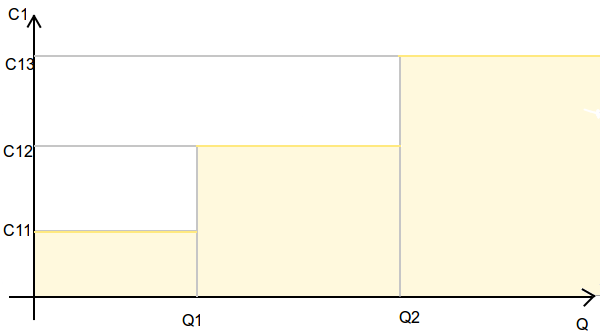
\includegraphics[scale=0.4,keepaspectratio=true]{img/7/7_QvsC1.png} 
\end{center}
Se sabe que para este modelo:
  \begin{equation}\label{7_CTE}CTE_i = bD + \frac{1}{2}qC_{1i}T + K\frac{D}{q} \end{equation}
  $$ q_{oi} = \sqrt{ \frac{2KD}{TC_{1i}}} $$
  $$ CTE_{oi} = bD + \sqrt{ 2KDC_{1i}T }$$

Con lo cual, se deduce la siguiente relacion entre variables:
 $$ C_{11} < C_{12} < C_{13} $$
 $$ q_{o1} > q_{o2} > q_{o3}$$
 $$ CTE_{o1} < CTE_{o2} < CTE_{o3} $$
 
El procedimiento a seguir para la búsqueda del costo total esperado mínimo es el siguiente: 
\begin{enumerate}
 \item si $q_{o1} < Q_1 \Rightarrow CTE_o = CTE_{o1}$ \\
      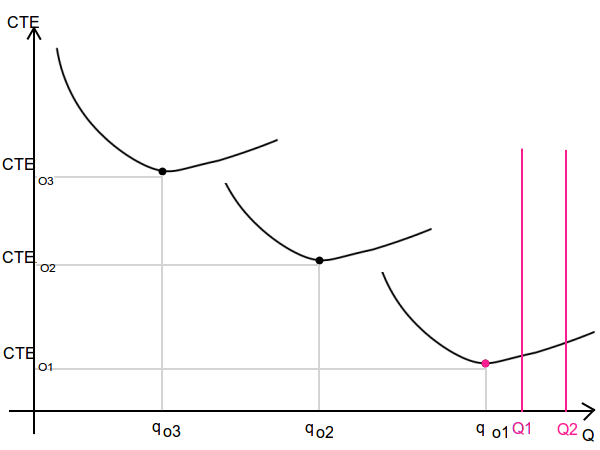
\includegraphics[scale=0.5,keepaspectratio=true]{img/7/7_QvsCTE_1.png} 
 \item sino, si $ q_{o2} < Q_1 \Rightarrow CTE_o = min( CTE(Q_1, C_{12}), CTE(Q_1, C_{11})$ \\
       Se entiende por $CTE(Q_i, C_{1i})$ el costo total esperado \eqref{7_CTE} evaluado en $Q_i$ y $C_{1i}$ \\
      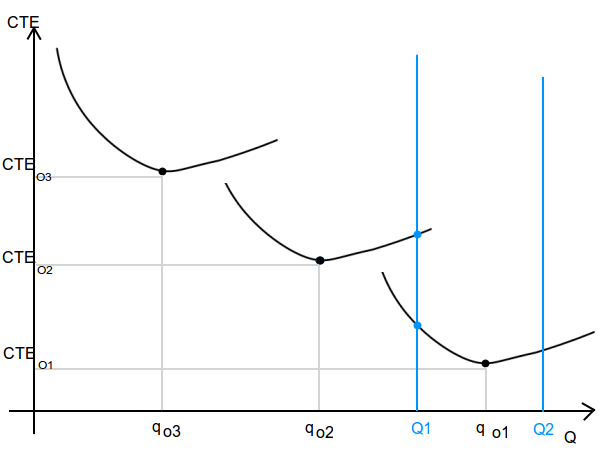
\includegraphics[scale=0.5,keepaspectratio=true]{img/7/7_QvsCTE_2.png} 
 \item sino, si $ Q_1 < q_{o2} < Q_2 \Rightarrow CTE_o = min( CTE_{o2}, CTE(Q_1, C_{11})) $ \\
      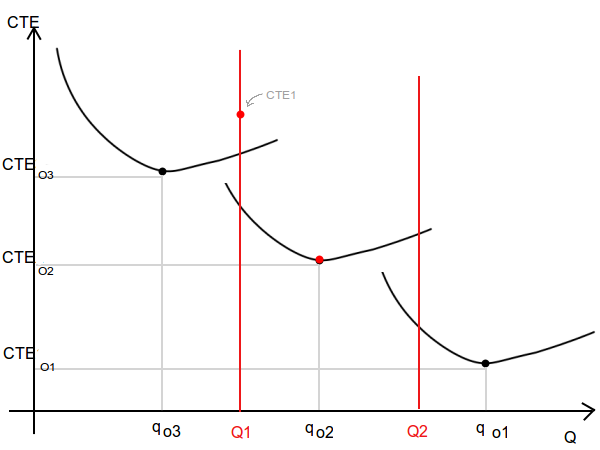
\includegraphics[scale=0.5,keepaspectratio=true]{img/7/7_QvsCTE_3.png} 
 \item sino, si $q_{o3} < Q_1 \Rightarrow CTE_o = min( CTE(Q_2, C_{12}), CTE(Q_2, C_{13}), CTE(Q_1, C_{11})) $ \\
      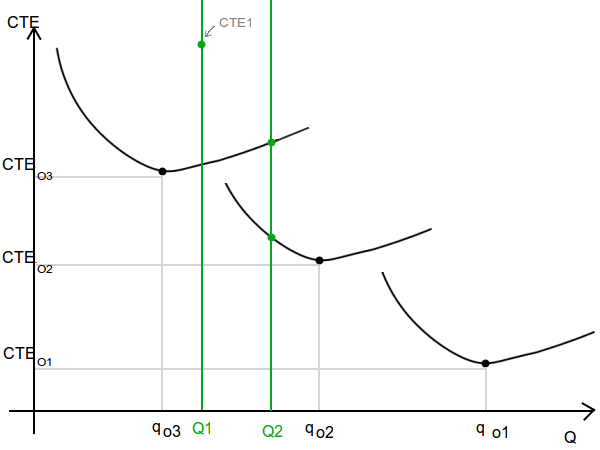
\includegraphics[scale=0.5,keepaspectratio=true]{img/7/7_QvsCTE_4.png} 
 \item sino, $q_{o3} > Q_2 \Rightarrow CTE_o = min(CTE_{o3},CTE(Q_2, C_{12}), CTE(Q_1, C_{11}) ) $ \\
      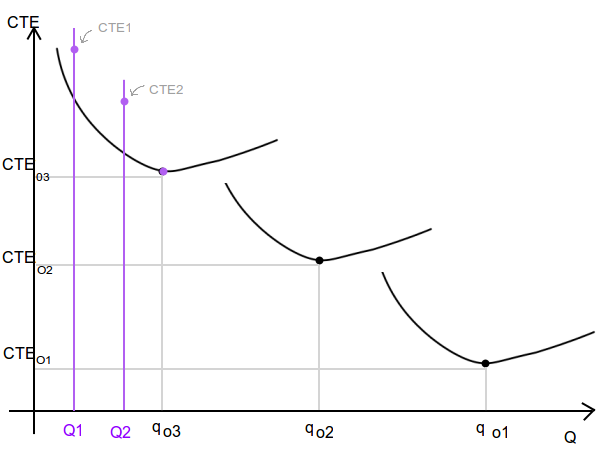
\includegraphics[scale=0.5,keepaspectratio=true]{img/7/7_QvsCTE_5.png} 
 \end{enumerate}

Para cada uno de estos casos, el costo total esperado en función de q está dado por la curva naranja, donde cada $CTE_i$ es válido dentro de su rango. 
\begin{enumerate}
 \item 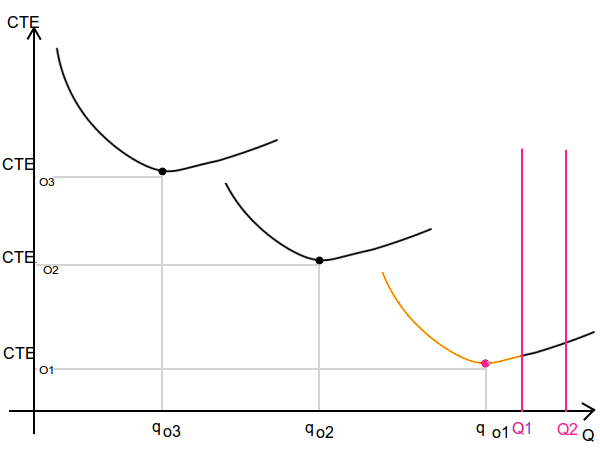
\includegraphics[scale=0.4,keepaspectratio=true]{img/7/7_QvsCTE_1B.png} 
 \item 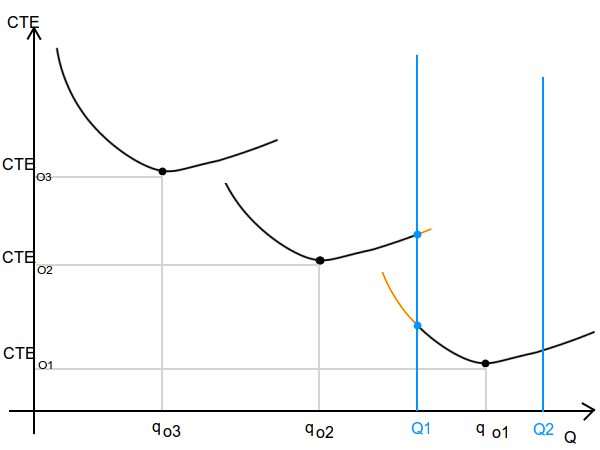
\includegraphics[scale=0.4,keepaspectratio=true]{img/7/7_QvsCTE_2B.png} 
 \item 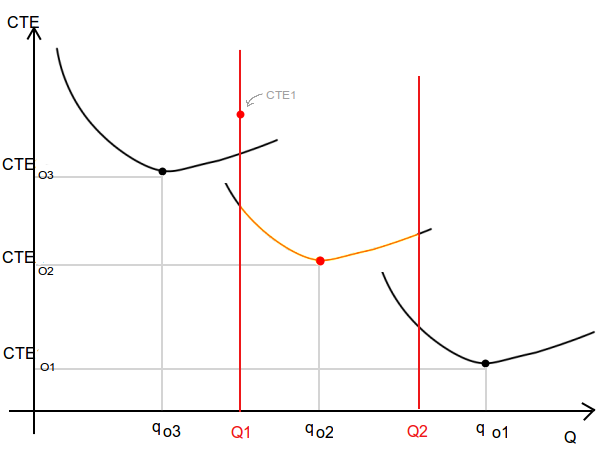
\includegraphics[scale=0.4,keepaspectratio=true]{img/7/7_QvsCTE_3B.png} 
 \item 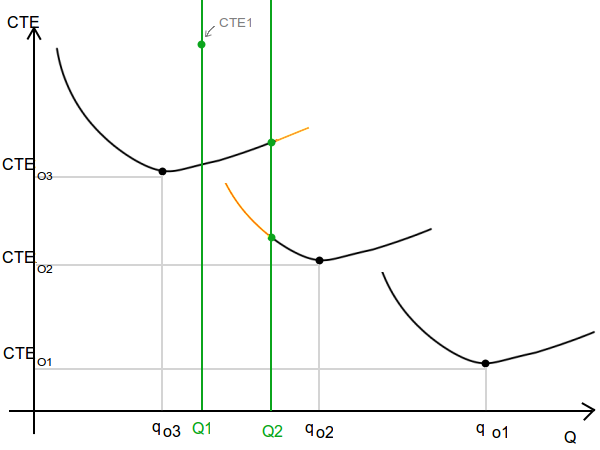
\includegraphics[scale=0.4,keepaspectratio=true]{img/7/7_QvsCTE_4B.png} 
 \item 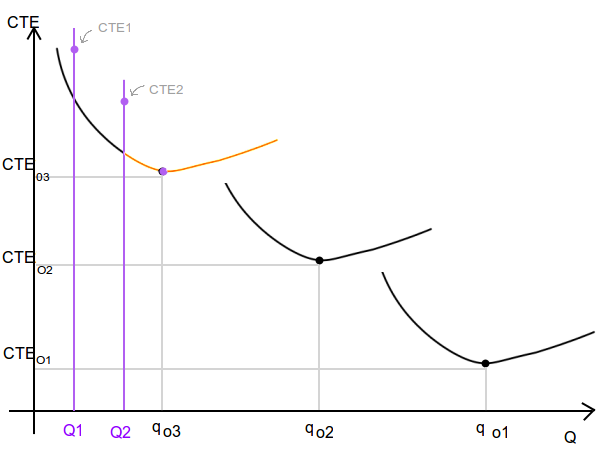
\includegraphics[scale=0.4,keepaspectratio=true]{img/7/7_QvsCTE_5B.png} 
\end{enumerate}


\paragraph{Ejercicio 8}
Se trata de un caso de modelo básico (ver ejercicio 1) de un solo ítem, demanda constante, agotamiento no admitido y con K creciente mediante la siguiente ley: 
\begin{center}
  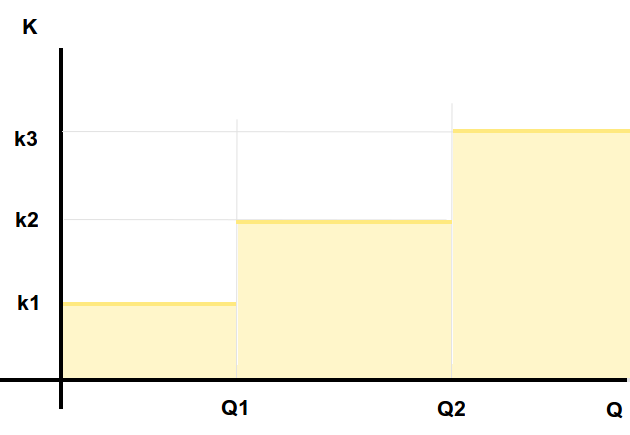
\includegraphics[scale=0.4,keepaspectratio=true]{img/8/8_QvsK.png} 
\end{center}

Se sabe que para este modelo:
  \begin{equation}\label{8_CTE}CTE_i = bD + \frac{1}{2}qC_1T + K_i \frac{D}{q} \end{equation}
  $$ q_{oi} = \sqrt{ \frac{2K_iD}{TC_1}} $$
  $$ CTE_{oi} = bD + \sqrt{ 2K_iDC_1T }$$

Con lo cual, se deduce la siguiente relacion entre variables:
 $$ k_1 < k_2 < k_3 $$
 $$ q_{o1} < q_{o2} < q_{o3}$$
 $$ CTE_{o1} < CTE_{o2} < CTE_{o3} $$
 
El procedimiento a seguir para la búsqueda del costo total esperado mínimo es el siguiente: 
\begin{enumerate}
 \item si $q_{o1} < Q_1 \Rightarrow CTE_o = CTE_{o1} $ \\
    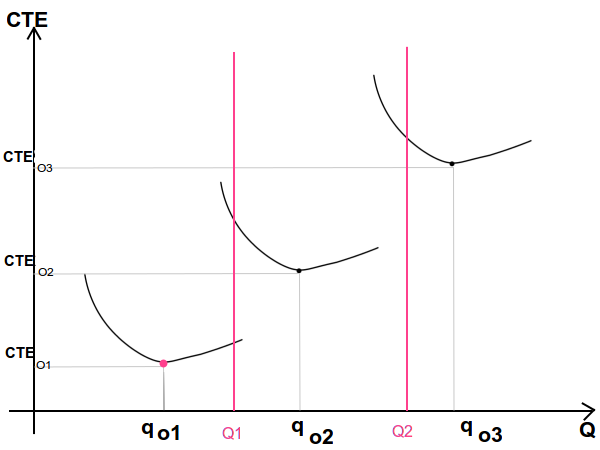
\includegraphics[scale=0.5,keepaspectratio=true]{img/8/8_QvsCTE_1.png} 
 \item sino, si $q_{o2} < Q_2 \Rightarrow CTE_o = min( CTE_{o2}, CTE(Q_1, k_1)) $ \\
      Se entiende por $CTE(Q_i, k_i)$ el costo total esperado \eqref{8_CTE} evaluado en $Q_i$ y $k_i$ \\
      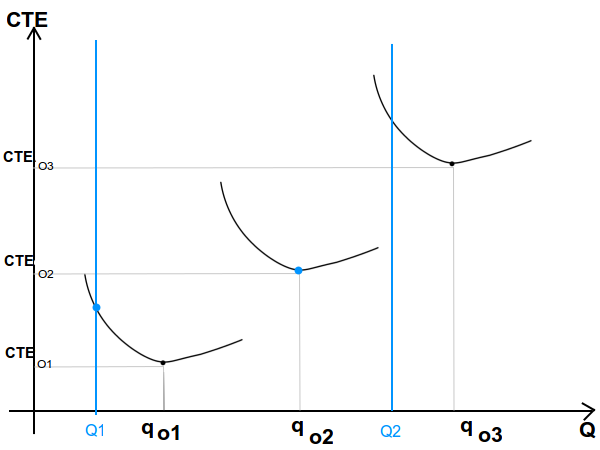
\includegraphics[scale=0.5,keepaspectratio=true]{img/8/8_QvsCTE_2.png} 
 \item sino, $q_{o3} > Q_2 \Rightarrow CTE_o = min( CTE_{o3}, CTE(Q_2, k_2), CTE(Q_1, k_1) )$ \\
      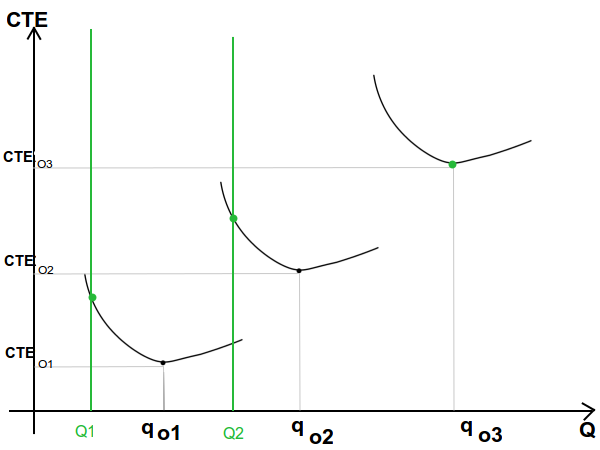
\includegraphics[scale=0.5,keepaspectratio=true]{img/8/8_QvsCTE_3.png} 
\end{enumerate}

Dado que cada curva es válida únicamente en un intervalo determinado por k, para cada caso el CTE en función de q está dado por la curva naranja.\\
\begin{enumerate}
  \item 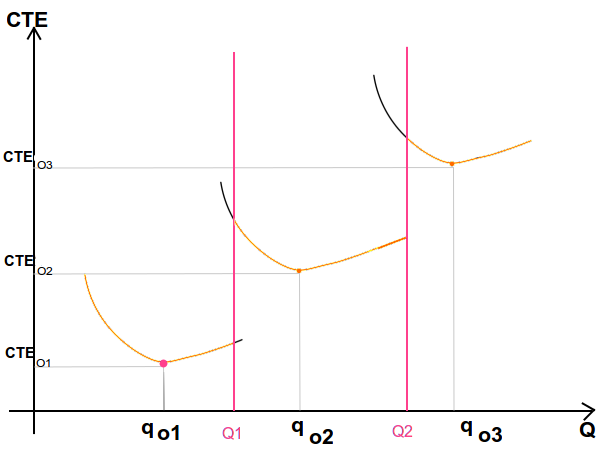
\includegraphics[scale=0.5,keepaspectratio=true]{img/8/8_QvsCTE_1b.png} 
  \item 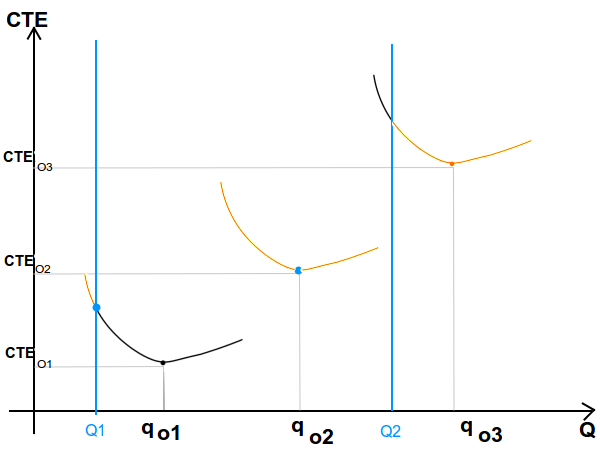
\includegraphics[scale=0.5,keepaspectratio=true]{img/8/8_QvsCTE_2b.png} 
  \item 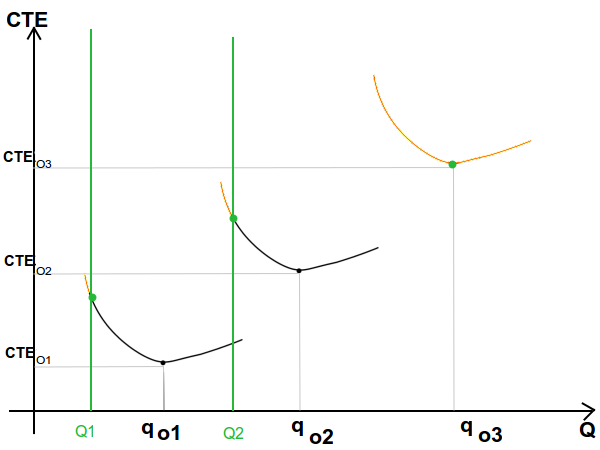
\includegraphics[scale=0.5,keepaspectratio=true]{img/8/8_QvsCTE_3b.png} 
\end{enumerate}

\end{document}
